\chapter{Aim of the Work}

As we discussed in Chapter \ref{chap:introduciton}, metamorphic
self-reconfigurable robots have several properties, which makes them an
appealing direction for future robotics trends. Those include versatility, fast
prototyping, and a high level of fault-tolerance. However, in the current
state-of-the-art, we are far from reaching these properties in practice. As we
showed in Chapter \ref{chap:state-of-the-art}, the research in this area is
broad and vivid. Nevertheless, there are plenty of challenges and open-problems
to tackle.

We want to focus on finding ways to control metamorphic robots in
a~fault-tolerant manner via distributed control in our research from all the
challenges that metamorphic robots present. We further describe our goals in the
following text.

\section{Evaluation Platform}

We want to demonstrate the solutions we will propose on physical robots, thus
making our research as reproducible as possible. Unfortunately, it is quite hard
in the area of robotics as one cannot easily download a robot and test our
solutions.

To achieve the best reproducibility as possible, it is crucial to use an easily
obtainable hardware platform. As we addressed in section
\ref{sec:reproducibility}, none of the platforms we discussed in chapter
\ref{chap:state-of-the-art} has manufacturing data (for mechanical construction
and PCBs) nor firmware publicly available. We also contacted the authors if they
are willing to share their design files or if there is a possibility of buying
their robots. Unfortunately, none of them responded positively. Only the authors
of SMORES \cite{DBLP:conf/iros/DaveyKY12} responded that it would be possible to
cooperate and try our solutions on their robots at their facility, which is not
convenient.

Therefore, as a by-product of the PhD study, we expect to develop an
open-hardware and open-source platform for metamorphic distributed robots. This
platform should serve as a tool for demonstrating our research outcomes, which
allows others to build their robots and reproduce our results easily. Also,
being the first open platform, it should serve as a research tool for others in
the area.

The platform, called the RoFI platform, is part of the study that was advanced
the most so far. We introduce it more in detail in Chapter \ref{chap:results}.

\section{Fault-Tolerant Distributed Control for RoFI}

We want to omit the reconfiguration part from the control and mainly focus on
designing fault-tolerant controllers that perform a given task without changing
the robot's shape. Therefore, as a result, distributed controllers are expected
to be designed since they should offer a more feasible path towards fault
tolerance than centralized approaches.

We expect to focus on a partial module malfunction since the system explosion is
more related to research about spatial localization and path planning than
distributed control. Similarly, complete module malfunction is probably better
solved by reconfiguration as distributed control has no other option how to deal
with a completely malfunctioned module than to ignore it.

A robot without sensors cannot interact with the environment and can only follow
hard-coded paths and, thus, can be used only in a highly controlled environment.
This is contrary to the overall motivation for metamorphic robots. Therefore
these robots have to feature a large number of sensors. In practice, one can
expect that some of these sensors can report faulty readings or become faulty.
Similarly, with a large number of communicating nodes, we can expect
communication errors to be present. Therefore, we want to propose a solution for
controlling metamorphic systems where the individual modules can feature
Byzantine faults originating from their sensors or faulty communication.
State-of-the-art does not cover these types of faults, as we could see in
Chapter \ref{chap:state-of-the-art}.

\section{Proposed Case Studies}

We expect two case studies to be performed during the PhD study to tackle the
challenges we stated above. That is to design a distributed controllers for
specific configurations, which allow the system to transport in space and be
fault-tolerant for partial module failures. After performing those case studies,
we would like to generalize the findings and introduce more general
approaches if applicable.

\begin{figure}[!t]
    \centering
    \begin{subfigure}[b]{0.45\textwidth}
        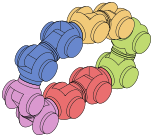
\includegraphics[width=\textwidth]{figures/ring_example.pdf}
        \caption{Loop Robot}
        \label{fig:example_roller}
    \end{subfigure}
    ~
    \begin{subfigure}[b]{0.45\textwidth}
        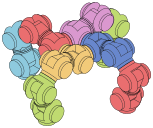
\includegraphics[width=\textwidth]{figures/spider_example.pdf}
        \caption{Walker Robot}
        \label{fig:example_spider}
    \end{subfigure}

    \caption{Examples of metamorphic systems for the case studies.}
\end{figure}

\subsection{Loop Robot}

In the first case study, we would like first to replicate the experiments
performed by \textcite{superbotroller} and
\textcite{DBLP:journals/ijrr/SastraCY09} on the RoFI platform. We will replicate
the experiments to get a baseline for our further research. In their
experiments, the authors use a loop robot to roll forward (see Figure
\ref{fig:example_roller} for an example of such a robot).

\textcite{superbotroller} perform two experiments on loop rolling: the first one
without any communication between modules (the modules act purely based on
observations from their accelerometers) and the second one with a~centralized
controller, where the master module controls the other modules.

\textcite{DBLP:journals/ijrr/SastraCY09} perform a centrally controlled
experiment on loop rolling. They leverage the dynamics of the system to move
faster compared to previous work. The controller uses accelerometers in the
modules as feedback.

Once we replicate the experiments, we would like to propose new controllers for
this configuration. The overall goal of the redesign is to explore the problem
of fault-tolerance on well-defined case and possibly find a concept of control
worth generalizing to an arbitrary configuration. We plan to introduce the
following improvements over the state-of-the-art:
\begin{itemize}
    \item We will transform the controller into a distributed one as the first
    step towards fault tolerance. This presents mainly a challenge in
    synchronization and information exchange -- especially sensor feedback. We
    would like to include inertial measurement units, obstacle distance, and
    torque feedback from the servomotors.
    \item Then we will remove the assumption that the individual
    modules report correct feedback. The controller should be able to deal with
    some number of units that provide incorrect feedback.
    \item If applicable, the controller should also be able to deal with some
    number of units with faulty joints.
    \item RoFI modules have a joint in the middle; therefore, we will implement
    steering, so the loop can turn left and right during motion. Processing the
    feedback loop for steering is the ultimate test on the quality of our
    control algorithms.
\end{itemize}

There are two ways to tackle the challenges given above. The first,
straightforward one and probably easier to handle, is to use leader-election
\cite{baca2016coordination} to elect a leading module. Then the system will
monitor whether the leader is alive, and if not, it will reelect a new one. The
leader can centrally collect sensor data and remotely control the
other modules. In this case, a faulty sensor could be handled in a byzantine way
(e.g., by an approach inspired by \textcite{DBLP:conf/osdi/CastroL99}).

The second approach is to use digital hormones (inspired by
\cite{DBLP:conf/cec/HamannSSC10, DBLP:conf/icra/MorenoG11}) for both control and
sensor feedback. This approach is more appealing as it leverages
self-reconfigurable robots' basics and possibly, should yield better results and
inherently tackle both sensors and actuators faults. However, as literature
shows, it is hard to apply.

Nevertheless, in both approaches, we would like to leverage system dynamics to
move faster and  be able to steer compared to state-of-the-art. Suitable
inspiration could be taken from cable robots which often resemble the
configuration used in this case study and thus, deal with similar problems in
locomotion \cite{DBLP:conf/iros/Hustig-SchultzS16, DBLP:conf/iros/CeraA18}. If
we manage to distribute sensor feedback well, it could open a possibility for
the loop to roll on bumpy terrain or stairs.

\subsection{Walker Robot}

The second case study should directly build on the results of the first one. Our
goal is to take a non-trivial configuration (e.g., the walker in Figure
\ref{fig:example_spider}) and apply our findings on it to perform synchronous
execution of the movement yielding locomotion by walking on a flat surface. The
goal of this study is to help us find generalizable approaches for control.

If we use the leader-election approach, this case study will focus on efficiency
of communication and scalability to large systems, possibly by introducing a
hierarchical approach (i.e., there is a separate leader for each limb of the
robot, and synchronization is only required among limb leaders and modules
belonging to the same limb).

If we use the hormone-based approach, this case study will probably focus on
designing a suitable hormone system for such configurations. We could explore
the possibility of introducing a library of hormone primitives that could be
composed together and simplify the design of complex hormone-based controllers,
which should significantly advance the state-of-the-art in control.

\section{Time Plan}

The plan of my future study and research activities is following:

\begin{description}[style=nextline,leftmargin=0.8cm]
    \item [now -- January 2023]
        Development and maintenance of the RoFI platform.
    \item [now -- January 2021]
        Replication of the loop robot experiments for RoFI.
    \item [January 2021]
        Doctoral exam and defense of this thesis proposal.
    \item [February 2021 -- June 2021]
        Designing the new controller for the loop configuration and
        investigation of fault-tolerant approaches.
    \item [June 2021 -- December 2022]
        Generalization of the outcomes of the loop configuration case study.
    \item[January 2022 -- August 2022]
        Application of the findings in context of complex configurations.
    \item[September 2022 -- January 2023]
        Summarizing my research and writing the PhD thesis.
    \item[January 2023]
        Defense of the PhD thesis.
\end{description}
